\documentclass[11pt,a4paper]{article}

% Packages
\usepackage[margin=2.5cm]{geometry}
\usepackage{microtype}
\usepackage{graphicx}
\usepackage{tikz}
\usetikzlibrary{shapes,arrows.meta,positioning,calc,fit,backgrounds,shadows.blur,decorations.pathmorphing,decorations.pathreplacing}
\usepackage{colortbl}
\usepackage{enumitem}
\usepackage{booktabs}
\usepackage{longtable}
\usepackage{hyperref}
\usepackage{xcolor}
\usepackage{fancyhdr}
\usepackage{titlesec}
\usepackage[most]{tcolorbox}
\usepackage{multicol}
\usepackage{amsmath,amssymb}
\usepackage{multirow}
\usepackage{setspace}
\usepackage{fontawesome5}
\usepackage{listings}
\usepackage{array}
\usepackage{tabularx}

% Spacing
\setlength{\parskip}{3pt plus 1pt minus 1pt}
\setlength{\parindent}{0pt}

% Colors
\definecolor{primary}{HTML}{0B4F6C}
\definecolor{secondary}{HTML}{1A8CA0}
\definecolor{accent}{HTML}{E74C3C}
\definecolor{lightbg}{HTML}{E8F6F8}
\definecolor{defbg}{HTML}{FDF2E9}
\definecolor{greenhl}{HTML}{1E8449}
\definecolor{purplehl}{HTML}{7D3C98}
\definecolor{codebg}{HTML}{F4F6F7}
\definecolor{tealhl}{HTML}{117A65}
\definecolor{warnbg}{HTML}{FEF9E7}

% Hyperref
\hypersetup{colorlinks=true, linkcolor=primary, urlcolor=secondary, citecolor=primary}

% Code listings style
\lstset{
  backgroundcolor=\color{codebg},
  basicstyle=\ttfamily\small,
  keywordstyle=\color{primary}\bfseries,
  stringstyle=\color{greenhl},
  commentstyle=\color{gray},
  breaklines=true,
  frame=l,
  framerule=2pt,
  rulecolor=\color{secondary!40},
  xleftmargin=8pt,
  framexleftmargin=6pt,
  aboveskip=6pt,
  belowskip=6pt
}

% Header/Footer
\pagestyle{fancy}
\fancyhf{}
\fancyhead[L]{\small\textcolor{primary}{\textbf{Parallel \& Distributed Computing --- BS CS}}}
\fancyhead[R]{\small\textcolor{primary}{Final-Term Exam Handout}}
\fancyfoot[C]{\small\thepage}
\fancyfoot[R]{\small\textcolor{gray!60}{July 2026}}
\renewcommand{\headrulewidth}{0.5pt}
\renewcommand{\footrulewidth}{0.3pt}

% Section formatting
\titleformat{\section}{\Large\bfseries\color{primary}}{\thesection}{0.6em}{}[\vspace{2pt}\titlerule]
\titleformat{\subsection}{\large\bfseries\color{secondary}}{\thesubsection}{0.5em}{}
\titleformat{\subsubsection}{\normalsize\bfseries\color{primary}}{\thesubsubsection}{0.5em}{}
\titlespacing*{\section}{0pt}{14pt}{8pt}
\titlespacing*{\subsection}{0pt}{10pt}{5pt}

% Part formatting
\titleformat{\part}[block]{\centering\huge\bfseries\color{primary}}{}{0pt}{}
\titlespacing*{\part}{0pt}{6pt}{10pt}

% Custom boxes
\newtcolorbox{definitionbox}[1][]{
  enhanced, breakable,
  colback=defbg, colframe=orange!60!black,
  colbacktitle=orange!70!black, coltitle=white,
  title={\faIcon{book}~#1}, fonttitle=\bfseries,
  boxrule=0pt, leftrule=4pt, arc=2pt,
  shadow={1mm}{-1mm}{0mm}{black!15},
  top=4pt, bottom=4pt, left=8pt, right=8pt
}
\newtcolorbox{conceptbox}[1][]{
  enhanced, breakable,
  colback=lightbg, colframe=secondary,
  colbacktitle=secondary, coltitle=white,
  title={\faIcon{lightbulb}~#1}, fonttitle=\bfseries,
  boxrule=0pt, leftrule=4pt, arc=2pt,
  shadow={1mm}{-1mm}{0mm}{black!15},
  top=4pt, bottom=4pt, left=8pt, right=8pt
}
\newtcolorbox{alertbox}[1][]{
  enhanced, breakable,
  colback=red!4, colframe=accent,
  colbacktitle=accent, coltitle=white,
  title={\faIcon{exclamation-triangle}~#1}, fonttitle=\bfseries,
  boxrule=0pt, leftrule=4pt, arc=2pt,
  shadow={1mm}{-1mm}{0mm}{black!12},
  top=3pt, bottom=3pt, left=8pt, right=8pt
}
\newtcolorbox{examplebox}[1][]{
  enhanced, breakable,
  colback=green!4, colframe=greenhl,
  colbacktitle=greenhl, coltitle=white,
  title={\faIcon{code}~#1}, fonttitle=\bfseries,
  boxrule=0pt, leftrule=4pt, arc=2pt,
  shadow={1mm}{-1mm}{0mm}{black!12},
  top=3pt, bottom=3pt, left=8pt, right=8pt
}
\newtcolorbox{formulabox}[1][]{
  enhanced, breakable,
  colback=purple!4, colframe=purplehl,
  colbacktitle=purplehl, coltitle=white,
  title={\faIcon{calculator}~#1}, fonttitle=\bfseries,
  boxrule=0pt, leftrule=4pt, arc=2pt,
  shadow={1mm}{-1mm}{0mm}{black!12},
  top=4pt, bottom=4pt, left=8pt, right=8pt
}

%=======================================================================
\begin{document}

% ---- Title Page ----
\begin{center}
\vspace*{0.4cm}
{\Huge\bfseries\textcolor{primary}{Parallel \& Distributed}}\\[8pt]
{\Huge\bfseries\textcolor{primary}{Computing}}\\[16pt]
{\color{secondary}\rule{0.65\textwidth}{1.5pt}}\\[14pt]
{\Large\textsc{Final-Term Comprehensive Handout}}\\[8pt]
{\large\textcolor{gray!70!black}{GPU \& CUDA $\bullet$ Advanced OpenMP/MPI $\bullet$ Parallel Algorithms $\bullet$ Consensus $\bullet$ Big Data $\bullet$ Cloud}}\\[6pt]
{\normalsize\textcolor{primary!70}{BS Computer Science \quad|\quad Cumulative (Full Semester) \quad|\quad July 2026}}
\vspace{0.3cm}
\end{center}

\begin{tcolorbox}[
  enhanced, colback=primary!6, colframe=primary,
  boxrule=1pt, arc=4pt, left=10pt, right=10pt, top=6pt, bottom=6pt
]
\textbf{\textcolor{primary}{\faIcon{clipboard-list}~Final-Term Exam Coverage (Cumulative):}} This handout is a \textbf{single, all-in-one study document} for the final examination. \textbf{Part~I} is a condensed recap of the midterm material (fundamentals, performance, synchronization, distributed-systems basics) delivered as quick-reference tables and formula boxes. \textbf{Part~II} covers all new final-term topics in depth: advanced shared-memory programming (OpenMP tasks, Pthreads), GPU/CUDA computing, advanced MPI, parallel algorithms, distributed coordination \& mutual exclusion, consensus (2PC/3PC/Paxos/Raft/PBFT), distributed transactions, MapReduce \& Spark, distributed file systems, cloud/virtualization/containers, and performance engineering. Focus on \textbf{formulae}, \textbf{definitions}, \textbf{algorithms}, and \textbf{comparison tables}.
\end{tcolorbox}
\vspace{6pt}
\tableofcontents
\newpage

%#######################################################################
\part{Part I --- Midterm Recap (Condensed)}
%#######################################################################

\begin{conceptbox}[How to use Part~I]
Part~I is a fast refresher, not a re-teaching. Each block collapses a midterm chapter into its exam-critical definitions, formulae, and comparison tables. If any row is unfamiliar, revisit the midterm handout (\texttt{PDC\_Handout.pdf}) before moving to Part~II.
\end{conceptbox}

%=======================================================================
\section{Fundamentals at a Glance}
%=======================================================================

\begin{definitionbox}[Core Definitions]
\textbf{Parallel Computing:} many calculations performed \textbf{simultaneously}; one problem split across multiple processors, usually tightly coupled.\\[3pt]
\textbf{Distributed Computing:} computation across multiple \textbf{networked, autonomous} computers that coordinate by \textbf{message passing} toward a common goal.\\[3pt]
\textbf{Concurrency vs Parallelism:} concurrency = \emph{dealing with} many things at once (composition/structure); parallelism = \emph{doing} many things at once (simultaneous execution).
\end{definitionbox}

\subsection{Parallel vs Distributed --- Summary}
\rowcolors{2}{white}{lightbg}
\begin{longtable}{@{}p{3.6cm}p{5.3cm}p{5.3cm}@{}}
\toprule
\rowcolor{primary!15}
\textbf{Aspect} & \textbf{Parallel} & \textbf{Distributed} \\
\midrule
\endhead
Memory & Shared or local, one site & Private per node, geographically spread \\
Communication & Shared variables / bus & Message passing over network \\
Clock & Often global/tight & No global clock; loose coupling \\
Failures & Rare, affect whole system & Frequent, \textbf{partial} failures normal \\
Primary goal & Speed (performance) & Scalability \& fault tolerance \\
Examples & Multi-core, GPU, OpenMP, CUDA & Clusters, Cloud, MPI, Hadoop \\
\bottomrule
\end{longtable}

\subsection{Flynn's Taxonomy \& Parallelism Types}
\rowcolors{2}{white}{lightbg}
\begin{longtable}{@{}p{1.7cm}p{6.0cm}p{5.5cm}@{}}
\toprule
\rowcolor{primary!15}
\textbf{Class} & \textbf{Meaning} & \textbf{Example} \\
\midrule
\endhead
SISD & Single instruction, single data (sequential) & Classic von Neumann CPU \\
SIMD & Single instruction, multiple data & GPU, AVX/SSE vector units \\
MISD & Multiple instruction, single data (rare) & Fault-tolerant pipelines \\
MIMD & Multiple instruction, multiple data & Multi-core, clusters \\
\bottomrule
\end{longtable}

\begin{itemize}[leftmargin=*, itemsep=2pt]
  \item \textbf{Data parallelism:} same operation over different data partitions (SIMD-style).
  \item \textbf{Task parallelism:} different operations run concurrently (MIMD-style).
  \item \textbf{Pipeline parallelism:} staged assembly line; stage $i$ processes item $n$ while stage $i{-}1$ processes $n{+}1$.
  \item \textbf{Memory models:} \textbf{Shared} (UMA/NUMA/ccNUMA), \textbf{Distributed} (message passing), \textbf{Hybrid} (multi-core nodes + interconnect, e.g.\ MPI+OpenMP).
\end{itemize}

%=======================================================================
\section{Performance Metrics --- Recap}
%=======================================================================

\begin{formulabox}[The Five Formulae You Must Know]
\begin{align*}
\text{Speedup:}\quad & S(p) = \frac{T_s}{T_p} & \text{Efficiency:}\quad & E(p) = \frac{S(p)}{p} = \frac{T_s}{p\,T_p}\\[6pt]
\text{Amdahl:}\quad & S(p) = \frac{1}{(1-f) + \dfrac{f}{p}} & \text{Amdahl limit:}\quad & S_{\max} = \frac{1}{1-f}\\[6pt]
\text{Gustafson:}\quad & S(p) = f\,p + (1-f) & &
\end{align*}
$T_s$ = serial time, $T_p$ = time on $p$ processors, $f$ = parallel fraction.
\end{formulabox}

\begin{alertbox}[Amdahl vs Gustafson --- the exam trap]
\textbf{Amdahl} fixes the \emph{problem size} $\Rightarrow$ speedup is capped by the serial fraction (pessimistic, models \textbf{strong scaling}). \textbf{Gustafson} lets the \emph{problem grow} with $p$ $\Rightarrow$ near-linear speedup is achievable (optimistic, models \textbf{weak scaling}). Same hardware, different assumption about workload.
\end{alertbox}

\rowcolors{2}{white}{lightbg}
\begin{longtable}{@{}p{3.8cm}p{4.4cm}p{5.0cm}@{}}
\toprule
\rowcolor{primary!15}
\textbf{Term} & \textbf{Definition} & \textbf{Note} \\
\midrule
\endhead
Linear speedup & $S = p$ & Ideal \\
Superlinear & $S > p$ & Rare; cache/memory effects \\
Strong scaling & Fixed problem, more $p$ & Bounded by Amdahl \\
Weak scaling & Problem grows with $p$ & Governed by Gustafson \\
Scale up (vertical) & Bigger machine & Limited by hardware \\
Scale out (horizontal) & More machines & Distributed systems path \\
\bottomrule
\end{longtable}

%=======================================================================
\section{Design, Synchronization \& Distributed Basics --- Recap}
%=======================================================================

\subsection{PCAM Design Methodology (Foster)}
\textbf{P}artitioning $\to$ \textbf{C}ommunication $\to$ \textbf{A}gglomeration $\to$ \textbf{M}apping. Start with the finest-grain tasks (domain or functional decomposition), identify data exchange, combine tasks to cut overhead, then place tasks on processors. \textbf{Load balancing} may be \emph{static} (fixed upfront) or \emph{dynamic} (runtime, e.g.\ work stealing / task queues).

\subsection{Synchronization Primitives}
\rowcolors{2}{white}{lightbg}
\begin{longtable}{@{}p{3.0cm}p{10.6cm}@{}}
\toprule
\rowcolor{primary!15}
\textbf{Primitive} & \textbf{Purpose} \\
\midrule
\endhead
Mutex & Binary lock; one holder at a time. \\
Semaphore & Integer with atomic P (wait/down) / V (signal/up); binary $\approx$ mutex, counting guards $n$ resources. \\
Monitor & High-level construct; auto mutual exclusion + condition variables (Java \texttt{synchronized}). \\
Barrier & All threads must arrive before any proceeds; phase separation. \\
\bottomrule
\end{longtable}

\begin{alertbox}[Critical Section \& Deadlock]
A \textbf{critical section} needs \textbf{Mutual Exclusion}, \textbf{Progress}, and \textbf{Bounded Waiting}. A \textbf{deadlock} requires all four Coffman conditions simultaneously: \textbf{Mutual Exclusion}, \textbf{Hold \& Wait}, \textbf{No Preemption}, \textbf{Circular Wait}. Break any one to prevent it (avoidance = Banker's Algorithm; also detect \& recover). Related pathologies: \textbf{livelock} (state changes, no progress) and \textbf{starvation} (perpetual denial).
\end{alertbox}

\subsection{Distributed Systems Basics}
\begin{itemize}[leftmargin=*, itemsep=2pt]
  \item \textbf{Goals:} transparency, openness, scalability, fault tolerance, performance. Transparency kinds: access, location, migration, replication, concurrency, failure.
  \item \textbf{CAP Theorem:} pick at most 2 of \{Consistency, Availability, Partition tolerance\}. Since partitions are inevitable, real systems choose \textbf{CP} (e.g.\ HBase, Zookeeper) or \textbf{AP} (e.g.\ Cassandra, DynamoDB).
  \item \textbf{Consistency models (strong$\to$weak):} strong, sequential, causal, eventual; plus client guarantees read-your-writes, monotonic reads.
  \item \textbf{Logical clocks:} \textbf{Lamport} ($a\to b \Rightarrow L(a){<}L(b)$, not iff) and \textbf{Vector clocks} ($V(a){<}V(b) \Leftrightarrow a\to b$, captures causality exactly).
  \item \textbf{Fault tolerance:} crash, omission, timing, response, \textbf{Byzantine} (arbitrary). BFT consensus needs $n \ge 3f+1$.
\end{itemize}

\begin{center}
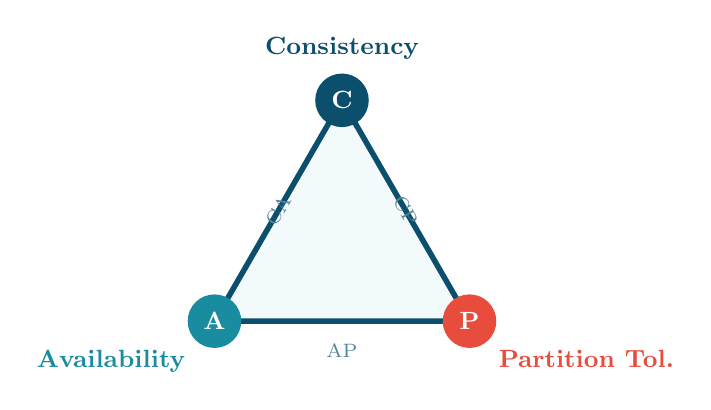
\begin{tikzpicture}[scale=0.85]
  \coordinate (C) at (90:2.2);
  \coordinate (A) at (210:2.2);
  \coordinate (P) at (330:2.2);
  \fill[lightbg, opacity=0.5] (C) -- (A) -- (P) -- cycle;
  \draw[very thick, primary, line width=2pt] (C) -- (A) -- (P) -- cycle;
  \fill[primary]   (C) circle (0.4cm); \node[white, font=\bfseries\small] at (C) {C};
  \fill[secondary] (A) circle (0.4cm); \node[white, font=\bfseries\small] at (A) {A};
  \fill[accent]    (P) circle (0.4cm); \node[white, font=\bfseries\small] at (P) {P};
  \node[font=\small\bfseries, primary, above=0.4cm]  at (C) {Consistency};
  \node[font=\small\bfseries, secondary, below left=0.35cm] at (A) {Availability};
  \node[font=\small\bfseries, accent, below right=0.35cm]  at (P) {Partition Tol.};
  \node[font=\scriptsize, align=center, primary!70, rotate=60]  at ($(C)!0.5!(A)$) {CA};
  \node[font=\scriptsize, align=center, primary!70, rotate=-60] at ($(C)!0.5!(P)$) {CP};
  \node[font=\scriptsize, align=center, primary!70]             at ($(A)!0.5!(P)+(0,-0.45)$) {AP};
\end{tikzpicture}
\end{center}

\newpage
%#######################################################################
\part{Part II --- Final-Term Core Topics}
%#######################################################################

%=======================================================================
\section{Advanced Shared-Memory Programming}
%=======================================================================

\subsection{OpenMP Beyond the Parallel For}
\begin{conceptbox}[The Fork--Join Model]
An OpenMP program runs as a single \textbf{master thread} that \textbf{forks} a team of threads at a \texttt{parallel} region and \textbf{joins} them at its end. Work-sharing constructs (\texttt{for}, \texttt{sections}, \texttt{single}, \texttt{task}) divide work among the team.
\end{conceptbox}

\subsubsection{Loop Scheduling}
The \texttt{schedule} clause controls how loop iterations map to threads --- crucial when iterations have \textbf{unequal cost}.
\rowcolors{2}{white}{lightbg}
\begin{longtable}{@{}p{3.2cm}p{6.5cm}p{3.9cm}@{}}
\toprule
\rowcolor{primary!15}
\textbf{Schedule} & \textbf{Behaviour} & \textbf{Best for} \\
\midrule
\endhead
\texttt{static, c} & Iterations split into fixed chunks of size \texttt{c}, assigned round-robin at compile/entry time. Lowest overhead. & Uniform iteration cost \\
\texttt{dynamic, c} & Threads grab chunks of size \texttt{c} from a shared queue as they finish. Balances load, higher overhead. & Irregular workloads \\
\texttt{guided, c} & Like dynamic but chunk size shrinks over time (large first, then small). & Unknown/irregular, tail balance \\
\texttt{runtime} & Decided by \texttt{OMP\_SCHEDULE} environment variable. & Tuning without recompiling \\
\texttt{auto} & Compiler/runtime chooses. & Let the system decide \\
\bottomrule
\end{longtable}

\subsubsection{Tasks and Sections}
\begin{examplebox}[OpenMP Tasks --- Irregular / Recursive Parallelism]
\begin{lstlisting}[language=C]
// Parallel recursive Fibonacci using tasks
int fib(int n) {
    if (n < 2) return n;
    int x, y;
    #pragma omp task shared(x)      // spawn independent task
    x = fib(n - 1);
    #pragma omp task shared(y)
    y = fib(n - 2);
    #pragma omp taskwait            // wait for both child tasks
    return x + y;
}
// Called once inside: #pragma omp parallel { #pragma omp single { fib(n); } }
\end{lstlisting}
\end{examplebox}

\begin{itemize}[leftmargin=*, itemsep=2pt]
  \item \texttt{task} --- creates a unit of deferred work placed in a pool; ideal for \textbf{unbounded/recursive} structures (trees, graphs, linked lists) where iteration count is unknown.
  \item \texttt{taskwait} --- suspends the current task until its child tasks complete.
  \item \texttt{sections} / \texttt{section} --- assign distinct code blocks to different threads (functional/task parallelism).
  \item \texttt{single} / \texttt{master} --- only one thread (or the master) executes the enclosed block.
\end{itemize}

\subsubsection{Data-Sharing \& Reductions}
\rowcolors{2}{white}{lightbg}
\begin{longtable}{@{}p{4.0cm}p{10.0cm}@{}}
\toprule
\rowcolor{primary!15}
\textbf{Clause} & \textbf{Meaning} \\
\midrule
\endhead
\texttt{shared(x)} & One instance of \texttt{x} shared by all threads. \\
\texttt{private(x)} & Each thread gets an uninitialised private copy. \\
\texttt{firstprivate(x)} & Private copy initialised to the value before the region. \\
\texttt{lastprivate(x)} & Value from the logically last iteration copied out. \\
\texttt{reduction(op:x)} & Private copies combined with \texttt{op} ($+$, $*$, \texttt{max}, \texttt{min}, \&\&) at the end. \\
\bottomrule
\end{longtable}

\begin{alertbox}[False Sharing --- a Silent Performance Killer]
When two threads repeatedly write to \textbf{different variables that share the same cache line}, the cache-coherence protocol keeps invalidating that line, forcing it to bounce between cores. The code is correct but slow. \textbf{Fix:} pad/align data so per-thread variables occupy separate cache lines, or use thread-local accumulation and combine at the end.
\end{alertbox}

\subsection{POSIX Threads (Pthreads)}
\begin{conceptbox}[Pthreads --- Explicit Low-Level Threading]
Where OpenMP is directive-based and implicit, \textbf{Pthreads} is a library giving you \textbf{explicit} control of thread creation, joining, and synchronisation --- more boilerplate, more control.
\end{conceptbox}

\begin{examplebox}[Pthreads: create, join, mutex]
\begin{lstlisting}[language=C]
#include <pthread.h>
pthread_mutex_t lock = PTHREAD_MUTEX_INITIALIZER;
long counter = 0;

void *worker(void *arg) {
    for (int i = 0; i < 100000; i++) {
        pthread_mutex_lock(&lock);     // enter critical section
        counter++;
        pthread_mutex_unlock(&lock);   // leave critical section
    }
    return NULL;
}
int main() {
    pthread_t t[4];
    for (int i = 0; i < 4; i++) pthread_create(&t[i], NULL, worker, NULL);
    for (int i = 0; i < 4; i++) pthread_join(t[i], NULL);  // wait for all
}
\end{lstlisting}
\end{examplebox}

\rowcolors{2}{white}{lightbg}
\begin{longtable}{@{}p{5.2cm}p{8.8cm}@{}}
\toprule
\rowcolor{primary!15}
\textbf{Pthreads Call} & \textbf{Role} \\
\midrule
\endhead
\texttt{pthread\_create} & Start a new thread running a given function. \\
\texttt{pthread\_join} & Block until a target thread finishes (collect it). \\
\texttt{pthread\_mutex\_lock/unlock} & Acquire / release a mutual-exclusion lock. \\
\texttt{pthread\_cond\_wait/signal} & Condition variables: sleep until a predicate holds / wake a waiter. \\
\texttt{pthread\_barrier\_wait} & Barrier synchronisation across threads. \\
\bottomrule
\end{longtable}

\subsection{Thread Pools \& Work Stealing}
\begin{itemize}[leftmargin=*, itemsep=2pt]
  \item \textbf{Thread pool:} a fixed set of worker threads pulling tasks from a shared queue --- avoids the cost of creating/destroying threads per task.
  \item \textbf{Work stealing:} each worker owns a double-ended queue (deque); it pushes/pops its own tasks from one end, and \textbf{idle workers steal} from the other end of a busy worker's deque. Used in Java \texttt{ForkJoinPool}, Intel TBB, Cilk. Excellent dynamic load balance with low contention.
\end{itemize}

\rowcolors{2}{white}{lightbg}
\begin{longtable}{@{}p{3.4cm}p{5.2cm}p{5.2cm}@{}}
\toprule
\rowcolor{primary!15}
\textbf{Feature} & \textbf{OpenMP} & \textbf{Pthreads} \\
\midrule
\endhead
Abstraction & High (directives) & Low (explicit library) \\
Effort & Incremental, small diff & Verbose, manual \\
Control & Coarser & Fine-grained \\
Load balancing & Built-in schedules & You implement it \\
Best when & Loop/data parallelism & Custom thread topologies \\
\bottomrule
\end{longtable}

%=======================================================================
\section{GPU Computing \& CUDA}
%=======================================================================

\begin{conceptbox}[Why GPUs?]
A CPU has a few powerful cores optimised for \textbf{latency} (fast single-thread, big caches, branch prediction). A GPU has \textbf{thousands} of simple cores optimised for \textbf{throughput}: run enormous numbers of threads so that memory-stalled threads are hidden by others that are ready. Ideal for \textbf{data-parallel}, arithmetic-heavy, regular workloads (matrices, images, neural networks).
\end{conceptbox}

\begin{center}
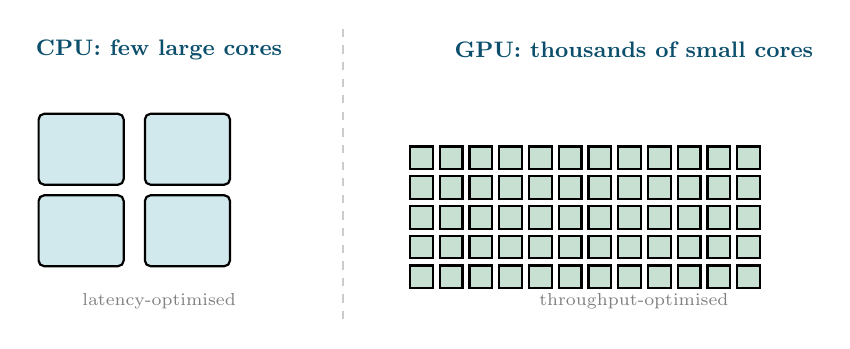
\begin{tikzpicture}[scale=0.9, transform shape,
  core/.style={rectangle, draw, thick, minimum size=0.32cm, inner sep=0pt},
  big/.style={rectangle, rounded corners=2pt, draw, thick, fill=secondary!20, minimum width=1.2cm, minimum height=1.0cm}
]
  % CPU
  \node[font=\small\bfseries, primary] at (-3.5, 2.7) {CPU: few large cores};
  \foreach \x in {0,1}{\foreach \y in {0,1}{
     \node[big] at (-4.6+\x*1.5, 0.15+\y*1.15) {};}}
  \node[font=\scriptsize, gray] at (-3.5, -0.85) {latency-optimised};
  % divider
  \draw[gray!40, thick, dashed] (-0.9,-1.1) -- (-0.9,3.0);
  % GPU
  \node[font=\small\bfseries, primary] at (3.2, 2.7) {GPU: thousands of small cores};
  \foreach \x in {0,...,11}{\foreach \y in {0,...,4}{
     \node[core, fill=greenhl!25] at (0.2+\x*0.42, -0.5+\y*0.42) {};}}
  \node[font=\scriptsize, gray] at (3.2, -0.85) {throughput-optimised};
\end{tikzpicture}
\end{center}

\subsection{The SIMT Execution Model}
\begin{definitionbox}[SIMT --- Single Instruction, Multiple Threads]
CUDA threads are grouped into \textbf{warps} of 32 that execute the \textbf{same instruction in lockstep} on different data. If threads in a warp take different branch paths (\textbf{warp divergence}), the paths are \emph{serialised}, hurting performance. Keep threads in a warp on the same control-flow path.
\end{definitionbox}

\subsection{Thread Hierarchy}
\begin{center}
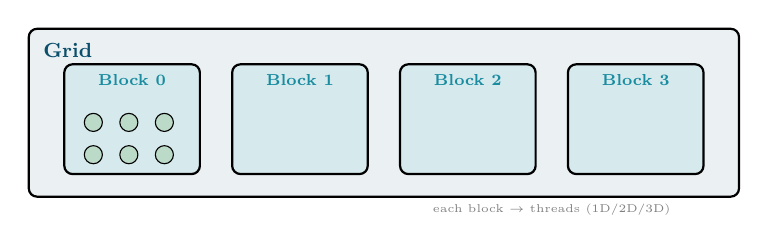
\begin{tikzpicture}[scale=0.82, transform shape,
  grid/.style={rectangle, rounded corners=3pt, draw, thick, fill=primary!8, minimum width=11cm, minimum height=2.6cm},
  blk/.style={rectangle, rounded corners=3pt, draw, thick, fill=secondary!18, minimum width=2.1cm, minimum height=1.7cm, align=center, font=\scriptsize\bfseries},
  th/.style={circle, draw, fill=greenhl!30, minimum size=0.28cm, inner sep=0pt}
]
  \node[grid] (g) at (0,0) {};
  \node[font=\small\bfseries, primary, anchor=north west] at (-5.4,1.2) {Grid};
  \foreach \i in {0,1,2,3}{
    \node[blk] (b\i) at (-3.9+\i*2.6, -0.1) {};
    \node[font=\scriptsize\bfseries, secondary] at (-3.9+\i*2.6, 0.5) {Block \i};
  }
  % threads inside block 0 (lower part, clear of the label)
  \foreach \x in {0,1,2}{\foreach \y in {0,1}{
    \node[th] at (-4.5+\x*0.55, -0.65+\y*0.5) {};}}
  \node[font=\tiny, gray, align=center] at (2.6,-1.5) {each block $\to$ threads (1D/2D/3D)};
\end{tikzpicture}
\end{center}
\begin{itemize}[leftmargin=*, itemsep=2pt]
  \item \textbf{Thread} --- runs the kernel; identified by \texttt{threadIdx}.
  \item \textbf{Block} --- group of threads that can cooperate via \textbf{shared memory} and \texttt{\_\_syncthreads()}; identified by \texttt{blockIdx}, sized by \texttt{blockDim}.
  \item \textbf{Grid} --- all blocks launched for one kernel; sized by \texttt{gridDim}.
  \item Global index: \texttt{int i = blockIdx.x * blockDim.x + threadIdx.x;}
\end{itemize}

\subsection{Memory Hierarchy}
\rowcolors{2}{white}{lightbg}
\begin{longtable}{@{}p{2.9cm}p{2.6cm}p{2.4cm}p{5.3cm}@{}}
\toprule
\rowcolor{primary!15}
\textbf{Memory} & \textbf{Scope} & \textbf{Speed} & \textbf{Notes} \\
\midrule
\endhead
Registers & Per thread & Fastest & Automatic variables \\
Shared memory & Per block & Very fast & On-chip; programmer-managed cache; use for data reuse \\
Global memory & Whole grid & Slow (high latency) & Main DRAM; coalesce accesses! \\
Constant memory & Read-only, all & Fast (cached) & Broadcast same value to warp \\
Local memory & Per thread & Slow & Register spills (actually in DRAM) \\
\bottomrule
\end{longtable}

\begin{examplebox}[CUDA Kernel --- Vector Addition]
\begin{lstlisting}[language=C++]
__global__ void vecAdd(const float *A, const float *B, float *C, int n) {
    int i = blockIdx.x * blockDim.x + threadIdx.x;  // global thread id
    if (i < n) C[i] = A[i] + B[i];                  // guard against overrun
}
int main() {
    float *dA, *dB, *dC;
    cudaMalloc(&dA, n*sizeof(float)); /* dB, dC similarly */
    cudaMemcpy(dA, hA, n*sizeof(float), cudaMemcpyHostToDevice);   // H->D
    int threads = 256, blocks = (n + threads - 1) / threads;       // ceil div
    vecAdd<<<blocks, threads>>>(dA, dB, dC, n);                    // launch
    cudaMemcpy(hC, dC, n*sizeof(float), cudaMemcpyDeviceToHost);   // D->H
    cudaFree(dA); /* ... */
}
\end{lstlisting}
\end{examplebox}

\subsection{Performance Levers}
\begin{itemize}[leftmargin=*, itemsep=2pt]
  \item \textbf{Memory coalescing:} consecutive threads should access consecutive global-memory addresses so the hardware merges them into one wide transaction.
  \item \textbf{Occupancy:} ratio of active warps to the maximum a Streaming Multiprocessor (SM) supports. Higher occupancy hides latency; limited by registers/shared-memory per block.
  \item \textbf{Host--device transfer:} the PCIe bus is a bottleneck --- minimise copies, keep data resident on the GPU, and overlap transfer with compute using \textbf{streams}.
  \item \textbf{Avoid divergence:} branch uniformly within a warp; avoid \texttt{if} that splits a warp.
\end{itemize}

\begin{alertbox}[CUDA vs OpenCL vs OpenMP-offload]
\textbf{CUDA} = NVIDIA-only, mature, best tooling. \textbf{OpenCL} = open, portable across GPUs/CPUs/FPGAs, more verbose. \textbf{OpenMP target}/\textbf{OpenACC} = directive-based GPU offloading, easiest to adopt. Exam angle: CUDA gives peak control/performance at the cost of portability.
\end{alertbox}

%=======================================================================
\section{Advanced Message Passing (MPI)}
%=======================================================================

\begin{conceptbox}[Recap: MPI Essentials]
\textbf{Rank} = process id $0..N{-}1$; \textbf{communicator} = a process group (\texttt{MPI\_COMM\_WORLD} = all). Point-to-point: \texttt{MPI\_Send}/\texttt{MPI\_Recv}. Collectives involve every process in a communicator. Final-term goes \emph{deeper}: communication modes, datatypes, topologies, one-sided, and hybrid models.
\end{conceptbox}

\subsection{Blocking, Non-Blocking \& Communication Modes}
\rowcolors{2}{white}{lightbg}
\begin{longtable}{@{}p{3.6cm}p{4.8cm}p{5.4cm}@{}}
\toprule
\rowcolor{primary!15}
\textbf{Call} & \textbf{Semantics} & \textbf{Use / Risk} \\
\midrule
\endhead
\texttt{MPI\_Send} (standard) & May buffer or block until receiver ready & Simple; deadlock risk if both send first \\
\texttt{MPI\_Ssend} (synchronous) & Returns only when receive has started & Guarantees rendezvous \\
\texttt{MPI\_Bsend} (buffered) & Copies to user buffer, returns immediately & Needs \texttt{MPI\_Buffer\_attach} \\
\texttt{MPI\_Isend/Irecv} & Non-blocking; returns a request handle & Overlap comm.\ with compute; must \texttt{MPI\_Wait}/\texttt{Test} \\
\bottomrule
\end{longtable}

\begin{alertbox}[Classic MPI Deadlock]
If every process calls a blocking \texttt{MPI\_Send} to its neighbour \emph{before} any \texttt{MPI\_Recv}, and buffers are full, all processes wait forever. \textbf{Fixes:} reorder send/recv (odd--even), use \texttt{MPI\_Sendrecv}, or use non-blocking \texttt{MPI\_Isend}/\texttt{MPI\_Irecv} then \texttt{MPI\_Waitall}.
\end{alertbox}

\subsection{Collective Operations (Deep Dive)}
\rowcolors{2}{white}{lightbg}
\begin{longtable}{@{}p{3.4cm}p{3.6cm}p{6.6cm}@{}}
\toprule
\rowcolor{primary!15}
\textbf{Pattern} & \textbf{MPI Call} & \textbf{Effect} \\
\midrule
\endhead
Barrier & \texttt{MPI\_Barrier} & All ranks synchronise. \\
Broadcast & \texttt{MPI\_Bcast} & Root's data copied to all ranks. \\
Scatter & \texttt{MPI\_Scatter} & Root splits an array, one chunk per rank. \\
Gather & \texttt{MPI\_Gather} & Root collects one chunk from each rank. \\
Allgather & \texttt{MPI\_Allgather} & Gather with result delivered to all ranks. \\
Reduce & \texttt{MPI\_Reduce} & Combine (sum/max/\ldots) into root. \\
Allreduce & \texttt{MPI\_Allreduce} & Reduce with result at all ranks (common in ML). \\
Reduce-scatter & \texttt{MPI\_Reduce\_scatter} & Reduce then scatter the result. \\
All-to-all & \texttt{MPI\_Alltoall} & Every rank sends distinct data to every rank (transpose). \\
Scan & \texttt{MPI\_Scan} & Prefix reduction across ranks. \\
\bottomrule
\end{longtable}

\begin{center}
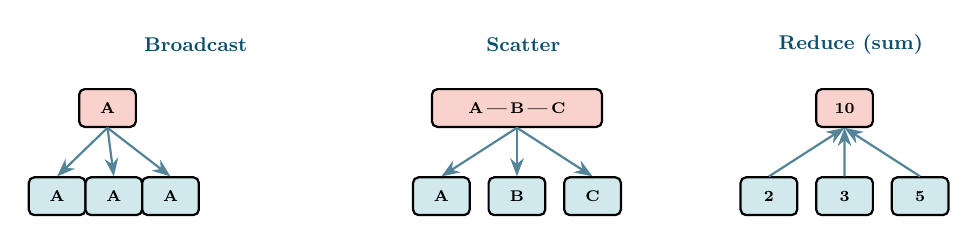
\begin{tikzpicture}[scale=0.8, transform shape,
  r/.style={rectangle, rounded corners=2pt, draw, thick, fill=#1, minimum width=0.9cm, minimum height=0.6cm, font=\scriptsize\bfseries},
  arr/.style={-{Stealth}, thick, primary!70}
]
  % Broadcast
  \node[font=\small\bfseries, primary] at (-4.2, 1.6) {Broadcast};
  \node[r=accent!25] (root) at (-5.6, 0.6) {A};
  \foreach \i in {0,1,2}{\node[r=secondary!20] (d\i) at (-6.4+\i*0.9, -0.8) {A};}
  \foreach \i in {0,1,2}{\draw[arr] (root.south) -- (d\i.north);}
  % Scatter
  \node[font=\small\bfseries, primary] at (1.0, 1.6) {Scatter};
  \node[r=accent!25, minimum width=2.7cm] (sr) at (0.9, 0.6) {A\,|\,B\,|\,C};
  \foreach \i/\L in {0/A,1/B,2/C}{\node[r=secondary!20] (s\i) at (-0.3+\i*1.2, -0.8) {\L};}
  \foreach \i in {0,1,2}{\draw[arr] (sr.south) -- (s\i.north);}
  % Reduce
  \node[font=\small\bfseries, primary] at (6.2, 1.6) {Reduce (sum)};
  \foreach \i/\L in {0/2,1/3,2/5}{\node[r=secondary!20] (g\i) at (4.9+\i*1.2, -0.8) {\L};}
  \node[r=accent!25] (gr) at (6.1, 0.6) {10};
  \foreach \i in {0,1,2}{\draw[arr] (g\i.north) -- (gr.south);}
\end{tikzpicture}
\end{center}

\subsection{Datatypes, Topologies \& One-Sided}
\begin{itemize}[leftmargin=*, itemsep=2pt]
  \item \textbf{Derived datatypes:} describe non-contiguous data (\texttt{MPI\_Type\_vector}, \texttt{\_contiguous}, \texttt{\_struct}) so you can send a matrix column or a struct in one call.
  \item \textbf{Virtual topologies:} impose a logical shape (\texttt{MPI\_Cart\_create} for grids/tori) that maps neighbours cleanly and lets the runtime optimise placement.
  \item \textbf{One-sided (RMA):} \texttt{MPI\_Put}/\texttt{MPI\_Get}/\texttt{MPI\_Accumulate} on a \textbf{window} of exposed memory --- the origin drives the transfer without the target actively receiving. Reduces synchronisation.
  \item \textbf{Communicators:} \texttt{MPI\_Comm\_split} partitions ranks into sub-groups for scoped collectives.
\end{itemize}

\begin{conceptbox}[Hybrid MPI + OpenMP]
Modern clusters are hierarchical: many multi-core nodes. The \textbf{hybrid model} uses \textbf{MPI between nodes} (distributed memory) and \textbf{OpenMP within a node} (shared memory). Benefits: fewer MPI ranks and messages, less memory replication, better use of intra-node bandwidth. This mirrors the \textbf{hybrid architecture} from Part~I.
\end{conceptbox}

%=======================================================================
\section{Parallel Algorithms}
%=======================================================================

\begin{definitionbox}[Work, Span \& Cost]
For a parallel computation: \textbf{Work} $W$ = total operations (time on 1 processor); \textbf{Span} (depth) $D$ = length of the longest dependency chain (time with $\infty$ processors). Then $T_p \ge \max(W/p,\, D)$ and parallelism $=W/D$. An algorithm is \textbf{cost-optimal} if $p \cdot T_p = \Theta(W_{\text{best serial}})$.
\end{definitionbox}

\subsection{Parallel Reduction \& Prefix Sum (Scan)}
\begin{itemize}[leftmargin=*, itemsep=2pt]
  \item \textbf{Reduction:} combine $n$ values (sum/max) via a balanced tree in $O(\log n)$ span, $O(n)$ work.
  \item \textbf{Prefix sum (scan):} output $y_i = x_0 \oplus x_1 \oplus \cdots \oplus x_i$. The \textbf{Hillis--Steele} scan runs in $O(\log n)$ steps ($O(n\log n)$ work); the work-efficient \textbf{Blelloch} scan uses up-sweep + down-sweep in $O(n)$ work, $O(\log n)$ span. Scan underpins stream compaction, sorting, and histograms.
\end{itemize}

\begin{center}
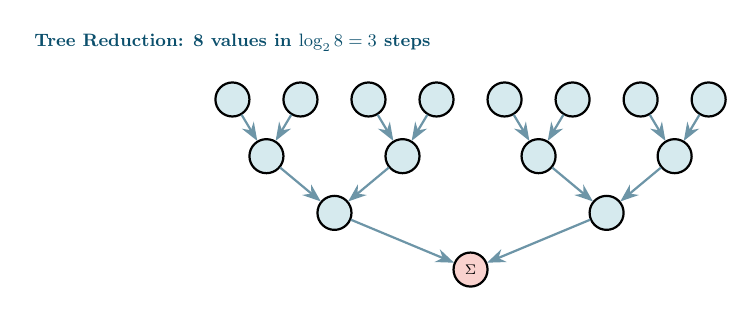
\begin{tikzpicture}[scale=0.72, transform shape,
  n/.style={circle, draw, thick, fill=secondary!18, minimum size=0.6cm, font=\scriptsize\bfseries},
  arr/.style={-{Stealth}, thick, primary!60}
]
  \node[font=\small\bfseries, primary] at (0,3.0) {Tree Reduction: 8 values in $\log_2 8 = 3$ steps};
  \foreach \i in {0,...,7}{\node[n] (a\i) at (\i*1.2, 2) {};}
  \foreach \i in {0,2,4,6}{\node[n] (b\i) at (\i*1.2+0.6, 1) {};}
  \foreach \i in {0,4}{\node[n] (c\i) at (\i*1.2+1.8, 0) {};}
  \node[n, fill=accent!25] (d) at (4.2, -1) {$\Sigma$};
  \draw[arr] (a0) -- (b0); \draw[arr] (a1) -- (b0);
  \draw[arr] (a2) -- (b2); \draw[arr] (a3) -- (b2);
  \draw[arr] (a4) -- (b4); \draw[arr] (a5) -- (b4);
  \draw[arr] (a6) -- (b6); \draw[arr] (a7) -- (b6);
  \draw[arr] (b0) -- (c0); \draw[arr] (b2) -- (c0);
  \draw[arr] (b4) -- (c4); \draw[arr] (b6) -- (c4);
  \draw[arr] (c0) -- (d); \draw[arr] (c4) -- (d);
\end{tikzpicture}
\end{center}

\subsection{Parallel Sorting}
\rowcolors{2}{white}{lightbg}
\begin{longtable}{@{}p{3.4cm}p{4.4cm}p{5.6cm}@{}}
\toprule
\rowcolor{primary!15}
\textbf{Algorithm} & \textbf{Idea} & \textbf{Complexity / Notes} \\
\midrule
\endhead
Odd--Even Transposition & Neighbour compare-exchange over odd/even phases & $O(n)$ phases; simple on arrays/rings \\
Bitonic Sort & Sort bitonic sequences via a fixed comparator network & $O(\log^2 n)$ depth; data-independent, great for GPUs/SIMD \\
Parallel Merge Sort & Divide, sort in parallel, parallel merge & $O(\log^2 n)$ span with parallel merge \\
Sample Sort & Pick splitters, bucket, sort buckets in parallel & Scales to clusters; near work-optimal \\
\bottomrule
\end{longtable}

\subsection{Parallel Matrix Multiplication --- Cannon's Algorithm}
\begin{conceptbox}[Cannon's Algorithm]
Multiply $A \times B$ on a $\sqrt{p} \times \sqrt{p}$ mesh of processors. Each processor holds one block of $A$ and $B$. After an \textbf{initial skew} (row $i$ of $A$ shifted left by $i$, column $j$ of $B$ shifted up by $j$), the algorithm alternates \textbf{multiply-accumulate} with \textbf{cyclic shifts} of blocks. Uses only $O(1)$ block storage per processor with nearest-neighbour communication --- memory-efficient and scalable versus a naive broadcast approach.
\end{conceptbox}

\begin{itemize}[leftmargin=*, itemsep=2pt]
  \item \textbf{Decomposition:} 2D block (checkerboard) partition of the matrices.
  \item \textbf{Communication:} only left/up neighbour shifts on a torus --- low, local, predictable.
  \item \textbf{Contrast:} Fox's algorithm broadcasts $A$ blocks along rows instead of skewing.
\end{itemize}

%=======================================================================
\section{Distributed Coordination \& Mutual Exclusion}
%=======================================================================

\begin{alertbox}[Why It's Hard]
In a distributed system there is \textbf{no shared memory} and \textbf{no global clock}. Mutexes and semaphores from Part~I don't apply directly --- mutual exclusion, election, and ordering must be built from \textbf{messages} alone, tolerating variable delays and failures.
\end{alertbox}

\subsection{Distributed Mutual Exclusion}
\rowcolors{2}{white}{lightbg}
\begin{longtable}{@{}p{3.3cm}p{5.6cm}p{2.4cm}p{2.1cm}@{}}
\toprule
\rowcolor{primary!15}
\textbf{Algorithm} & \textbf{Mechanism} & \textbf{Msgs / entry} & \textbf{Weakness} \\
\midrule
\endhead
Centralized & A coordinator grants a single token/lock on request & 3 & Coordinator is bottleneck/SPOF \\
Token Ring & A token circulates; holder may enter CS & 1 to $\infty$ & Token loss; latency \\
Ricart--Agrawala & Timestamped requests; enter after all others reply OK & $2(N{-}1)$ & Every node must reply; failure-sensitive \\
Maekawa & Request permission from a voting \emph{quorum} $\approx \sqrt{N}$ & $\approx 3\sqrt{N}$ & Deadlock possible; needs care \\
\bottomrule
\end{longtable}

\begin{conceptbox}[Ricart--Agrawala (Lamport-clock based)]
To enter the critical section, a process broadcasts a \textbf{timestamped REQUEST} to all others. A receiver replies \textbf{OK} immediately unless it is in (or wants) the CS with an \emph{earlier} timestamp, in which case it \textbf{defers} the reply. A process enters once it has received OK from \textbf{all} $N{-}1$ peers. Ties broken by process id. Guarantees mutual exclusion and fairness using logical clocks.
\end{conceptbox}

\subsection{Leader Election}
\begin{center}
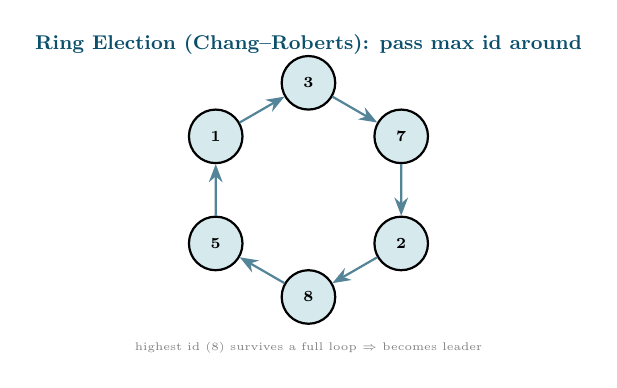
\begin{tikzpicture}[scale=0.8, transform shape,
  n/.style={circle, draw, thick, fill=secondary!18, minimum size=0.85cm, font=\scriptsize\bfseries},
  arr/.style={-{Stealth}, thick, primary!70}
]
  \node[font=\small\bfseries, primary] at (0,2.3) {Ring Election (Chang--Roberts): pass max id around};
  \foreach \i/\ang/\id in {0/90/3, 1/30/7, 2/-30/2, 3/-90/8, 4/-150/5, 5/150/1}{
     \node[n] (p\i) at (\ang:1.7) {\id};}
  \foreach \i/\j in {0/1,1/2,2/3,3/4,4/5,5/0}{\draw[arr] (p\i) -- (p\j);}
  \node[font=\tiny, gray] at (0,-2.5) {highest id (8) survives a full loop $\Rightarrow$ becomes leader};
\end{tikzpicture}
\end{center}

\rowcolors{2}{white}{lightbg}
\begin{longtable}{@{}p{3.4cm}p{10.4cm}@{}}
\toprule
\rowcolor{primary!15}
\textbf{Algorithm} & \textbf{How the leader is chosen} \\
\midrule
\endhead
Bully & A node that notices the leader is down sends ELECTION to all \emph{higher}-id nodes; if none answer it declares itself leader (COORDINATOR); higher nodes ``bully'' lower ones. $O(N^2)$ msgs worst case. \\
Chang--Roberts (Ring) & Each node forwards the maximum id it has seen around a logical ring; the node whose id returns to it is the leader. $O(N)$--$O(N^2)$ msgs. \\
\bottomrule
\end{longtable}

\subsection{Distributed Deadlock}
\begin{itemize}[leftmargin=*, itemsep=2pt]
  \item Detected via a global \textbf{Wait-For Graph (WFG)}; a cycle indicates deadlock.
  \item Techniques: centralized detection, edge-chasing (\textbf{Chandy--Misra--Haas} probe messages), and \textbf{timeouts}.
  \item Prevention via ordering / \textbf{wait--die} \& \textbf{wound--wait} timestamp schemes (from distributed transactions).
\end{itemize}

%=======================================================================
\section{Distributed Consensus \& Agreement}
%=======================================================================

\begin{definitionbox}[The Consensus Problem]
A set of processes must \textbf{agree on a single value} despite failures, satisfying: \textbf{Agreement} (no two decide differently), \textbf{Validity} (the value was proposed), and \textbf{Termination} (every correct process eventually decides).
\end{definitionbox}

\begin{alertbox}[FLP Impossibility Result]
In a \textbf{purely asynchronous} system, \textbf{no deterministic} consensus algorithm can guarantee termination if even \textbf{one} process may crash --- you cannot distinguish a slow process from a dead one. Practical systems escape FLP using \textbf{timeouts} (partial synchrony), \textbf{randomization}, or \textbf{failure detectors}.
\end{alertbox}

\subsection{Atomic Commit: Two-Phase \& Three-Phase Commit}
\begin{center}
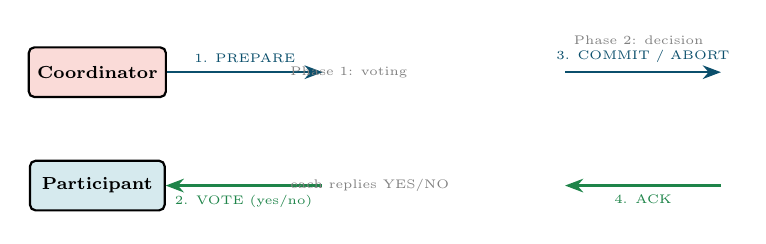
\begin{tikzpicture}[scale=0.9, transform shape,
  actor/.style={rectangle, rounded corners=2pt, draw, thick, fill=#1, minimum width=1.9cm, minimum height=0.7cm, font=\scriptsize\bfseries, align=center},
  msg/.style={-{Stealth}, thick}
]
  \node[actor=accent!20] (c) at (-4.2, 1.4) {Coordinator};
  \node[actor=secondary!18] (p1) at (-4.2, -0.2) {Participant};
  % phase 1
  \draw[msg, primary] (c.east) -- ++(2.2,0) node[midway, above, font=\tiny] {1. PREPARE};
  \draw[msg, greenhl] (p1.east) ++(2.2,0) -- (p1.east) node[midway, below, font=\tiny] {2. VOTE (yes/no)};
  \node[font=\tiny, gray, align=left, anchor=west] at (-1.6, 1.4) {Phase 1: voting};
  \node[font=\tiny, gray, align=left, anchor=west] at (-1.6, -0.2) {each replies YES/NO};
  % phase 2
  \draw[msg, primary] (2.4,1.4) -- ++(2.2,0) node[midway, above, font=\tiny] {3. COMMIT / ABORT};
  \draw[msg, greenhl] (4.6,-0.2) -- ++(-2.2,0) node[midway, below, font=\tiny] {4. ACK};
  \node[font=\tiny, gray, align=left, anchor=west] at (2.4, 1.85) {Phase 2: decision};
\end{tikzpicture}
\end{center}

\begin{itemize}[leftmargin=*, itemsep=2pt]
  \item \textbf{2PC:} Phase 1 coordinator asks all to \textbf{PREPARE}; if \emph{all} vote YES it broadcasts \textbf{COMMIT}, else \textbf{ABORT}. Guarantees atomicity but is \textbf{blocking}: if the coordinator crashes after PREPARE, participants holding locks can wait indefinitely.
  \item \textbf{3PC:} inserts a \textbf{pre-commit} phase so participants can reach a timeout-based decision without the coordinator, making it \textbf{non-blocking} under crash faults --- but it fails under network partitions and is rarely used in practice.
\end{itemize}

\subsection{Paxos}
\begin{conceptbox}[Paxos Roles \& Phases]
Roles: \textbf{Proposers}, \textbf{Acceptors}, \textbf{Learners}. Two phases: \textbf{(1) Prepare/Promise} --- a proposer picks a number $n$, asks a majority of acceptors to promise not to accept anything numbered $<n$; \textbf{(2) Accept/Accepted} --- the proposer asks acceptors to accept value $v$ with number $n$. A value chosen by a \textbf{majority quorum} is final. Safe despite crashes/message loss; famously subtle. \textbf{Multi-Paxos} amortises phase~1 by electing a stable leader.
\end{conceptbox}

\subsection{Raft --- Understandable Consensus}
\begin{center}
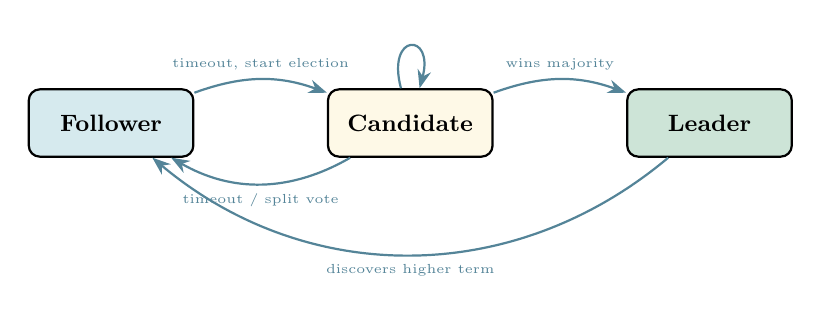
\begin{tikzpicture}[scale=0.95, transform shape,
  st/.style={rectangle, rounded corners=4pt, draw, thick, fill=#1, minimum width=2.2cm, minimum height=0.9cm, font=\small\bfseries, align=center},
  arr/.style={-{Stealth}, thick, primary!70}
]
  \node[st=secondary!18] (f) at (-4, 0) {Follower};
  \node[st=warnbg] (c) at (0, 0) {Candidate};
  \node[st=greenhl!22] (l) at (4, 0) {Leader};
  \draw[arr, bend left=20] (f) to node[above, font=\tiny] {timeout, start election} (c);
  \draw[arr, bend left=20] (c) to node[above, font=\tiny] {wins majority} (l);
  \draw[arr, bend left=30] (c) to node[below, font=\tiny] {timeout / split vote} (f);
  \draw[arr, bend left=40] (l) to node[below, font=\tiny] {discovers higher term} (f);
  \draw[arr, loop above] (c) to node[above, font=\tiny] {} (c);
\end{tikzpicture}
\end{center}
\begin{itemize}[leftmargin=*, itemsep=2pt]
  \item \textbf{Leader election:} time is divided into \textbf{terms}; a candidate that wins a majority vote becomes leader and sends periodic \textbf{heartbeats}.
  \item \textbf{Log replication:} clients talk only to the leader, which appends entries and replicates them; an entry is \textbf{committed} once stored on a majority, then applied to the state machine.
  \item \textbf{Safety:} a leader must have the most up-to-date log to be elected, guaranteeing committed entries are never lost. Equivalent power to Multi-Paxos, designed for \textbf{understandability}.
\end{itemize}

\subsection{Byzantine Fault Tolerance (PBFT)}
\begin{alertbox}[Byzantine Consensus]
When up to $f$ nodes may act \textbf{arbitrarily/maliciously} (send conflicting messages), consensus needs $\mathbf{n \ge 3f + 1}$ nodes. \textbf{PBFT} (Practical BFT) reaches agreement in three phases --- \textbf{pre-prepare $\to$ prepare $\to$ commit} --- tolerating $f$ Byzantine faults with $O(n^2)$ messaging. This underlies permissioned blockchains; public blockchains instead use \textbf{Proof-of-Work / Proof-of-Stake} (probabilistic Nakamoto consensus).
\end{alertbox}

\rowcolors{2}{white}{lightbg}
\begin{longtable}{@{}p{2.8cm}p{2.6cm}p{3.2cm}p{4.6cm}@{}}
\toprule
\rowcolor{primary!15}
\textbf{Protocol} & \textbf{Fault model} & \textbf{Quorum / bound} & \textbf{Property} \\
\midrule
\endhead
2PC & Crash & All must vote & Atomic but blocking \\
3PC & Crash & Majority + timeout & Non-blocking; fails on partition \\
Paxos / Raft & Crash (non-Byz.) & Majority ($> n/2$) & Safe, live under partial synchrony \\
PBFT & Byzantine & $n \ge 3f+1$ & Tolerates malicious nodes \\
\bottomrule
\end{longtable}

%=======================================================================
\section{Distributed Transactions \& Data}
%=======================================================================

\begin{definitionbox}[ACID vs BASE]
\textbf{ACID} (traditional RDBMS): \textbf{A}tomicity, \textbf{C}onsistency, \textbf{I}solation, \textbf{D}urability --- strong guarantees, harder to scale out.\\[3pt]
\textbf{BASE} (many NoSQL): \textbf{B}asically \textbf{A}vailable, \textbf{S}oft state, \textbf{E}ventual consistency --- trade strict consistency for availability and scale. This is the CAP trade-off in practice.
\end{definitionbox}

\subsection{Concurrency Control \& Quorums}
\begin{itemize}[leftmargin=*, itemsep=2pt]
  \item \textbf{Isolation} via two-phase locking (2PL), timestamp ordering, or \textbf{MVCC} (multi-version concurrency control --- readers don't block writers).
  \item \textbf{Quorum consistency:} with $N$ replicas, a write acknowledged by $W$ and a read querying $R$ replicas give \textbf{strong consistency when} $\mathbf{R + W > N}$ (read and write sets overlap). Tuning $R,W$ trades latency vs consistency (Dynamo-style).
  \item \textbf{Conflict resolution} for multi-master writes: last-writer-wins, version vectors, or CRDTs (conflict-free replicated data types).
\end{itemize}

\subsection{Replication Strategies \& NoSQL Models}
\rowcolors{2}{white}{lightbg}
\begin{longtable}{@{}p{3.5cm}p{4.6cm}p{5.4cm}@{}}
\toprule
\rowcolor{primary!15}
\textbf{NoSQL type} & \textbf{Data model} & \textbf{Examples} \\
\midrule
\endhead
Key--Value & Hash map of key $\to$ blob & Redis, DynamoDB, Riak \\
Document & JSON/BSON documents & MongoDB, CouchDB \\
Column-family & Sparse wide rows by column families & Cassandra, HBase \\
Graph & Nodes + edges + properties & Neo4j, JanusGraph \\
\bottomrule
\end{longtable}

\begin{itemize}[leftmargin=*, itemsep=2pt]
  \item \textbf{Primary--Backup (master--slave):} one writer, replicas follow; simple, primary is a bottleneck.
  \item \textbf{Multi-Primary:} several writers; needs conflict resolution.
  \item \textbf{Sharding + Replication:} partition data across nodes (horizontal scale) \emph{and} replicate each shard (fault tolerance) --- the standard large-scale pattern.
\end{itemize}

%=======================================================================
\section{MapReduce \& Big-Data Frameworks}
%=======================================================================

\begin{conceptbox}[The MapReduce Model (Google, 2004)]
Express a computation as two functions: \textbf{Map}$(k_1,v_1) \to \text{list}(k_2,v_2)$ processes input in parallel; the framework \textbf{shuffles/sorts} by $k_2$; \textbf{Reduce}$(k_2,\text{list}(v_2)) \to \text{list}(v_3)$ aggregates per key. The framework handles \textbf{parallelization, data distribution, fault tolerance, and scheduling} --- the programmer writes only map \& reduce.
\end{conceptbox}

\begin{center}
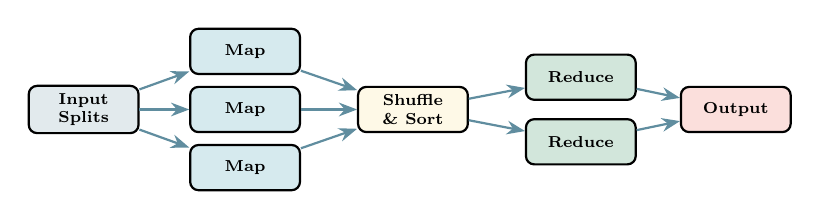
\begin{tikzpicture}[scale=0.82, transform shape,
  b/.style={rectangle, rounded corners=3pt, draw, thick, fill=#1, minimum width=1.7cm, minimum height=0.7cm, font=\scriptsize\bfseries, align=center},
  arr/.style={-{Stealth}, thick, primary!65}
]
  \node[b=primary!12] (in) at (-6.5,0) {Input\\Splits};
  \node[b=secondary!18] (m1) at (-4,0.9) {Map};
  \node[b=secondary!18] (m2) at (-4,0) {Map};
  \node[b=secondary!18] (m3) at (-4,-0.9) {Map};
  \node[b=warnbg] (sh) at (-1.4,0) {Shuffle\\ \& Sort};
  \node[b=greenhl!20] (r1) at (1.2,0.5) {Reduce};
  \node[b=greenhl!20] (r2) at (1.2,-0.5) {Reduce};
  \node[b=accent!18] (out) at (3.6,0) {Output};
  \foreach \m in {m1,m2,m3}{\draw[arr] (in) -- (\m); \draw[arr] (\m) -- (sh);}
  \draw[arr] (sh) -- (r1); \draw[arr] (sh) -- (r2);
  \draw[arr] (r1) -- (out); \draw[arr] (r2) -- (out);
\end{tikzpicture}
\end{center}

\begin{examplebox}[Word Count --- the ``Hello World'' of MapReduce (pseudocode)]
\begin{lstlisting}[language=Python]
def map(doc_name, text):
    for word in text.split():
        emit(word, 1)            # (word, 1) pairs

def reduce(word, counts):
    emit(word, sum(counts))      # total occurrences per word
\end{lstlisting}
\end{examplebox}

\subsection{Hadoop Ecosystem}
\begin{itemize}[leftmargin=*, itemsep=2pt]
  \item \textbf{HDFS} --- distributed storage (see \S13).
  \item \textbf{YARN} --- cluster resource manager / job scheduler.
  \item \textbf{MapReduce engine} --- batch execution on HDFS data (disk-heavy: writes intermediate results to disk between stages).
  \item Higher-level: \textbf{Hive} (SQL-on-Hadoop), \textbf{Pig}, \textbf{HBase} (column store).
\end{itemize}

\subsection{Apache Spark}
\begin{conceptbox}[RDDs and In-Memory Computing]
Spark's core abstraction is the \textbf{RDD (Resilient Distributed Dataset)} --- an immutable, partitioned collection computed in parallel. Spark keeps data \textbf{in memory} across operations, making iterative and interactive workloads far faster than disk-based MapReduce (often $10$--$100\times$).
\end{conceptbox}

\begin{itemize}[leftmargin=*, itemsep=2pt]
  \item \textbf{Transformations} (\texttt{map}, \texttt{filter}, \texttt{flatMap}, \texttt{reduceByKey}, \texttt{join}) are \textbf{lazy} --- they build a DAG (lineage) but don't execute.
  \item \textbf{Actions} (\texttt{collect}, \texttt{count}, \texttt{save}, \texttt{reduce}) trigger execution of the DAG.
  \item \textbf{Fault tolerance} via \textbf{lineage}: a lost partition is recomputed from its parent RDDs --- no need to replicate all data.
  \item Libraries: \textbf{Spark SQL}/DataFrames, \textbf{MLlib}, \textbf{GraphX}, \textbf{Structured Streaming}.
\end{itemize}

\begin{examplebox}[Spark Word Count (PySpark)]
\begin{lstlisting}[language=Python]
counts = (sc.textFile("hdfs://input.txt")
            .flatMap(lambda line: line.split())   # transformation (lazy)
            .map(lambda w: (w, 1))                 # transformation (lazy)
            .reduceByKey(lambda a, b: a + b))      # transformation (lazy)
counts.saveAsTextFile("hdfs://output")             # ACTION -> runs the DAG
\end{lstlisting}
\end{examplebox}

\rowcolors{2}{white}{lightbg}
\begin{longtable}{@{}p{3.6cm}p{5.0cm}p{5.0cm}@{}}
\toprule
\rowcolor{primary!15}
\textbf{Aspect} & \textbf{Hadoop MapReduce} & \textbf{Apache Spark} \\
\midrule
\endhead
Data flow & Disk between stages & In-memory (RDD) \\
Speed & Slower (I/O bound) & $10$--$100\times$ for iterative jobs \\
Model & Map + Reduce only & Rich operators + DAG \\
Fault tolerance & Re-run tasks, replication & RDD lineage recomputation \\
Best for & Huge one-pass batch & Iterative, interactive, ML, streaming \\
\bottomrule
\end{longtable}

%=======================================================================
\section{Distributed File Systems \& Storage}
%=======================================================================

\begin{conceptbox}[GFS / HDFS Design Principles]
Built for \textbf{commodity hardware} where failures are the norm. Files are split into large \textbf{blocks} (HDFS default 128\,MB) spread across nodes and \textbf{replicated} (default $3\times$) for fault tolerance. Optimised for \textbf{large streaming reads} and \textbf{append/write-once}, not small random writes.
\end{conceptbox}

\begin{center}
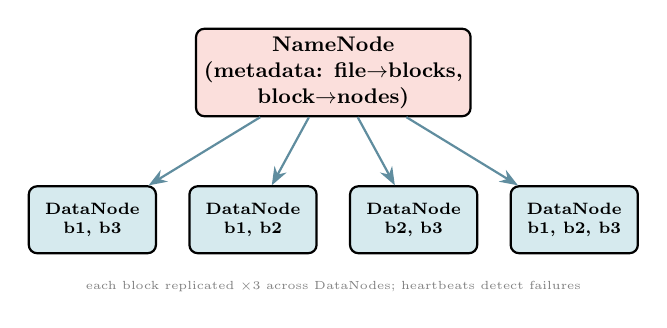
\begin{tikzpicture}[scale=0.85, transform shape,
  nn/.style={rectangle, rounded corners=3pt, draw, thick, fill=accent!18, minimum width=3.2cm, minimum height=0.9cm, font=\small\bfseries, align=center},
  dn/.style={rectangle, rounded corners=3pt, draw, thick, fill=secondary!18, minimum width=1.9cm, minimum height=1.0cm, font=\scriptsize\bfseries, align=center},
  arr/.style={-{Stealth}, thick, primary!65}
]
  \node[nn] (nn) at (0, 1.6) {NameNode\\(metadata: file$\to$blocks,\\block$\to$nodes)};
  \node[dn] (d1) at (-3.6, -0.6) {DataNode\\ b1, b3};
  \node[dn] (d2) at (-1.2, -0.6) {DataNode\\ b1, b2};
  \node[dn] (d3) at (1.2, -0.6)  {DataNode\\ b2, b3};
  \node[dn] (d4) at (3.6, -0.6)  {DataNode\\ b1, b2, b3};
  \foreach \d in {d1,d2,d3,d4}{\draw[arr] (nn) -- (\d);}
  \node[font=\tiny, gray] at (0,-1.6) {each block replicated $\times 3$ across DataNodes; heartbeats detect failures};
\end{tikzpicture}
\end{center}

\begin{itemize}[leftmargin=*, itemsep=2pt]
  \item \textbf{NameNode (master):} holds all metadata (namespace, block locations); a \textbf{single point of failure} historically --- mitigated by a standby NameNode + journal.
  \item \textbf{DataNodes (workers):} store actual block replicas; send periodic \textbf{heartbeats} + block reports.
  \item \textbf{Rack awareness:} replicas placed across racks so a rack failure doesn't lose data; \textbf{re-replication} restores the replication factor after a node dies.
  \item \textbf{Object storage} (Amazon S3, Ceph): flat namespace of objects with rich metadata; the backbone of cloud data lakes.
\end{itemize}

%=======================================================================
\section{Cloud, Virtualization \& Containers}
%=======================================================================

\begin{definitionbox}[Virtualization]
Abstracting physical hardware so multiple isolated \textbf{virtual machines (VMs)} share one physical host, each with its own OS. Managed by a \textbf{hypervisor}: \textbf{Type 1} (bare-metal, e.g.\ ESXi, Xen, Hyper-V) runs directly on hardware; \textbf{Type 2} (hosted, e.g.\ VirtualBox, VMware Workstation) runs atop a host OS.
\end{definitionbox}

\begin{center}
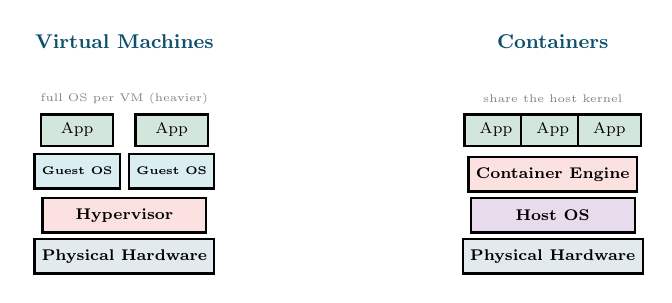
\begin{tikzpicture}[scale=0.8, transform shape,
  layer/.style={rectangle, draw, thick, minimum width=2.6cm, minimum height=0.55cm, font=\scriptsize\bfseries, align=center},
  app/.style={rectangle, draw, thick, fill=greenhl!20, minimum width=1.15cm, minimum height=0.5cm, font=\scriptsize}
]
  % VM stack
  \node[font=\small\bfseries, primary] at (-3.4, 3.4) {Virtual Machines};
  \node[layer, fill=primary!12] (hw1) at (-3.4,0) {Physical Hardware};
  \node[layer, fill=accent!16] (hyp) at (-3.4,0.65) {Hypervisor};
  \node[layer, fill=secondary!16, minimum width=1.35cm, font=\tiny\bfseries] (g1) at (-4.15,1.35) {Guest OS};
  \node[layer, fill=secondary!16, minimum width=1.35cm, font=\tiny\bfseries] (g2) at (-2.65,1.35) {Guest OS};
  \node[app] at (-4.15,2.0) {App}; \node[app] at (-2.65,2.0) {App};
  % Container stack
  \node[font=\small\bfseries, primary] at (3.4, 3.4) {Containers};
  \node[layer, fill=primary!12] (hw2) at (3.4,0) {Physical Hardware};
  \node[layer, fill=purplehl!18] (host) at (3.4,0.65) {Host OS};
  \node[layer, fill=accent!16] (eng) at (3.4,1.3) {Container Engine};
  \node[app, minimum width=1.0cm] at (2.5,2.0) {App}; \node[app, minimum width=1.0cm] at (3.4,2.0) {App}; \node[app, minimum width=1.0cm] at (4.3,2.0) {App};
  \node[font=\tiny, gray, align=center] at (3.4,2.5) {share the host kernel};
  \node[font=\tiny, gray, align=center] at (-3.4,2.5) {full OS per VM (heavier)};
\end{tikzpicture}
\end{center}

\begin{alertbox}[VMs vs Containers]
\textbf{VMs} virtualize \emph{hardware} --- each carries a full guest OS: strong isolation, heavier (GBs, slow boot). \textbf{Containers} (Docker) virtualize the \emph{OS} --- they share the host kernel and package just the app + dependencies: lightweight (MBs, sub-second start), less isolation. Containers made \textbf{microservices} and elastic scaling practical.
\end{alertbox}

\begin{itemize}[leftmargin=*, itemsep=2pt]
  \item \textbf{Docker:} build once (image), run anywhere; layered images, registries.
  \item \textbf{Kubernetes:} orchestrates containers across a cluster --- scheduling, self-healing, service discovery, load balancing, auto-scaling (pods, deployments, services).
  \item \textbf{Serverless / FaaS} (AWS Lambda): run functions on demand; no server management, pay per invocation, auto-scales to zero.
  \item \textbf{Service models (recap):} \textbf{IaaS} (VMs/storage) $\to$ \textbf{PaaS} (managed runtime) $\to$ \textbf{SaaS} (ready apps); deployment models: public, private, hybrid, community.
\end{itemize}

\begin{conceptbox}[Cluster vs Grid vs Cloud]
\textbf{Cluster:} tightly-coupled homogeneous nodes on a LAN, one administrative domain (HPC). \textbf{Grid:} geographically dispersed, heterogeneous, multi-domain resource sharing. \textbf{Cloud:} on-demand, elastic, virtualized resources billed pay-as-you-go, hiding the infrastructure.
\end{conceptbox}

%=======================================================================
\section{Performance Engineering \& Analysis}
%=======================================================================

\begin{definitionbox}[Arithmetic Intensity \& the Roofline Model]
\textbf{Arithmetic (operational) intensity} $I = \dfrac{\text{FLOPs}}{\text{bytes moved}}$ (flop/byte). The \textbf{Roofline model} bounds attainable performance:
\[
P_{\text{attainable}} = \min\big(\,P_{\text{peak}},\; I \times B_{\text{mem}}\,\big)
\]
where $P_{\text{peak}}$ is peak compute (FLOP/s) and $B_{\text{mem}}$ is peak memory bandwidth (byte/s). Low-$I$ kernels are \textbf{memory-bound} (on the slanted roof); high-$I$ kernels are \textbf{compute-bound} (under the flat roof).
\end{definitionbox}

\begin{center}
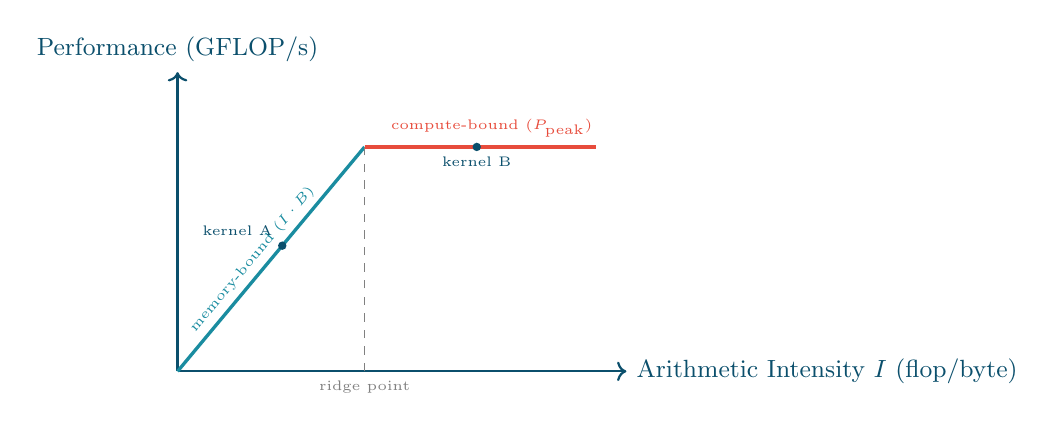
\begin{tikzpicture}[scale=0.95]
  \draw[->, thick, primary] (0,0) -- (6,0) node[right, font=\small] {Arithmetic Intensity $I$ (flop/byte)};
  \draw[->, thick, primary] (0,0) -- (0,4) node[above, font=\small] {Performance (GFLOP/s)};
  % slanted memory-bound roof
  \draw[secondary, very thick] (0,0) -- (2.5,3);
  % flat compute-bound roof
  \draw[accent, very thick] (2.5,3) -- (5.6,3);
  \node[font=\tiny, secondary, rotate=50] at (1.0,1.5) {memory-bound ($I\cdot B$)};
  \node[font=\tiny, accent] at (4.2,3.25) {compute-bound ($P_{\text{peak}}$)};
  \draw[dashed, gray] (2.5,0) -- (2.5,3);
  \node[font=\tiny, gray, below] at (2.5,0) {ridge point};
  \fill[primary] (1.4,1.68) circle (1.6pt) node[above left, font=\tiny] {kernel A};
  \fill[primary] (4.0,3.0) circle (1.6pt) node[below, font=\tiny] {kernel B};
\end{tikzpicture}
\end{center}

\subsection{Diagnosing and Improving Performance}
\begin{itemize}[leftmargin=*, itemsep=2pt]
  \item \textbf{Profile first:} tools like \texttt{gprof}, \texttt{perf}, Intel VTune, NVIDIA Nsight, Scalasca reveal hotspots; never optimise by guessing.
  \item \textbf{Overlap communication \& computation:} use non-blocking MPI / CUDA streams so transfers hide behind useful work.
  \item \textbf{Improve locality:} blocking/tiling for cache, avoid false sharing, coalesce memory.
  \item \textbf{Reduce synchronization:} fewer barriers/locks; prefer reductions and lock-free structures.
  \item \textbf{Amdahl in practice:} attack the \emph{largest serial fraction} first; a fast section already near its limit yields little.
\end{itemize}

\begin{alertbox}[Sources of Parallel Overhead]
Speedup falls short of ideal because of: \textbf{communication} (latency + bandwidth), \textbf{synchronization} (idle waiting at barriers/locks), \textbf{load imbalance}, \textbf{redundant computation}, and \textbf{serial bottlenecks}. Communication cost model: $T_{\text{comm}} = t_s + \dfrac{m}{B}$ (startup latency $t_s$ + message size $m$ / bandwidth $B$).
\end{alertbox}

%=======================================================================
\section{Emerging \& Applied Topics}
%=======================================================================

\begin{itemize}[leftmargin=*, itemsep=3pt]
  \item \textbf{Heterogeneous computing:} combine CPUs + GPUs + FPGAs/TPUs; match each task to the best accelerator. Basis of modern AI/HPC (e.g.\ GPU clusters training large models with data/model parallelism + Allreduce).
  \item \textbf{Edge \& fog computing:} push computation toward data sources (IoT devices, gateways) to cut latency and bandwidth; cloud handles heavy aggregation.
  \item \textbf{Green / energy-aware computing:} performance-per-watt matters as much as raw speed; DVFS, consolidation, and efficient scheduling reduce energy.
  \item \textbf{HPC $\leftrightarrow$ Cloud convergence:} elastic cloud HPC, containers on supercomputers, and serverless data pipelines blur the old boundaries.
\end{itemize}

%#######################################################################
% Back matter: consolidated formula & fact sheet
%#######################################################################
\newpage
\section*{Final-Term Formula \& Fact Sheet}
\addcontentsline{toc}{section}{Final-Term Formula \& Fact Sheet}

\begin{center}
\begin{tcolorbox}[
  enhanced, colback=primary!5, colframe=primary,
  boxrule=1pt, arc=4pt, width=\textwidth,
  title={\faIcon{star}~Key Formulae \& Numbers}, fonttitle=\bfseries\large,
  colbacktitle=primary, coltitle=white
]
\begin{multicols}{2}
\textbf{\textcolor{primary}{Performance:}}
\begin{itemize}[leftmargin=*, itemsep=2pt]
  \item Speedup $S = T_s/T_p$; \; Efficiency $E = S/p$
  \item Amdahl: $S = \dfrac{1}{(1-f)+f/p}$, \; $S_{\max}=\dfrac{1}{1-f}$
  \item Gustafson: $S = fp + (1-f)$
  \item Roofline: $P = \min(P_{\text{peak}},\, I\cdot B)$
  \item Comm.: $T_{\text{comm}} = t_s + m/B$
  \item Work/Span: $T_p \ge \max(W/p,\, D)$
\end{itemize}

\columnbreak

\textbf{\textcolor{primary}{Distributed rules of thumb:}}
\begin{itemize}[leftmargin=*, itemsep=2pt]
  \item Quorum strong consistency: $R + W > N$
  \item Byzantine (PBFT): $n \ge 3f + 1$
  \item Crash consensus quorum: $> n/2$
  \item CAP: choose 2 of C, A, P
  \item Ricart--Agrawala: $2(N{-}1)$ msgs/entry
  \item Maekawa quorum size $\approx \sqrt{N}$
  \item HDFS block 128\,MB, replication $\times 3$
\end{itemize}
\end{multicols}
\end{tcolorbox}
\end{center}

\vspace{6pt}
\begin{center}
\begin{tcolorbox}[
  enhanced, colback=orange!5, colframe=orange!70!black,
  boxrule=1pt, arc=4pt, width=\textwidth,
  title={\faIcon{tasks}~High-Yield Comparison Grid}, fonttitle=\bfseries,
  colbacktitle=orange!70!black, coltitle=white
]
\rowcolors{2}{white}{orange!8}
\begin{tabular}{@{}p{3.4cm}p{5.2cm}p{5.2cm}@{}}
\toprule
\rowcolor{orange!20}
\textbf{Pair} & \textbf{Left} & \textbf{Right} \\
\midrule
OpenMP vs Pthreads & Directive, implicit, easy & Library, explicit, fine control \\
CPU vs GPU & Few latency cores & Thousands throughput cores \\
2PC vs 3PC & Blocking on coord.\ crash & Non-blocking, fails on partition \\
Paxos/Raft vs PBFT & Crash faults, majority & Byzantine, $n\ge 3f{+}1$ \\
Hadoop vs Spark & Disk, map+reduce & In-memory RDD, DAG \\
VM vs Container & Full guest OS, heavy & Shares kernel, light \\
Amdahl vs Gustafson & Fixed size, strong scaling & Growing size, weak scaling \\
\bottomrule
\end{tabular}
\end{tcolorbox}
\end{center}

\vspace{6pt}
\begin{conceptbox}[Exam Strategy]
Expect: (1) a \textbf{numeric} problem (speedup/efficiency/Amdahl/Gustafson or quorum); (2) a \textbf{compare-and-contrast} (from the grid above); (3) an \textbf{algorithm trace} (Ricart--Agrawala, 2PC, Raft election, MapReduce word count, Cannon's shift); (4) a \textbf{define \& explain} on GPU/CUDA, CAP, consensus, or containers. Always state \textbf{assumptions}, show \textbf{formula $\to$ substitution $\to$ result}, and label \textbf{diagrams}.
\end{conceptbox}

\vspace{6pt}
\begin{center}
\textcolor{gray!60}{\small --- End of Handout --- BS CS $|$ Parallel \& Distributed Computing $|$ Final-Term (Cumulative) $|$ July 2026 ---}
\end{center}

\end{document}
